\documentclass[12pt,a4paper]{article}

\usepackage{graphicx}% Include figure files
\usepackage{dcolumn}% Align table columns on decimal point
\usepackage{bm}% bold math
%\usepackage{hyperref}% add hypertext capabilities
%\usepackage[mathlines]{lineno}% Enable numbering of text and display math
%\linenumbers\relax % Commence numbering lines

%\usepackage[showframe,%Uncomment any one of the following lines to test 
%%scale=0.7, marginratio={1:1, 2:3}, ignoreall,% default settings
%%text={7in,10in},centering,
%%margin=1.5in,
%%total={6.5in,8.75in}, top=1.2in, left=0.9in, includefoot,
%%height=10in,a5paper,hmargin={3cm,0.8in},
%]{geometry}

\usepackage{multicol}%Para hacer varias columnas
\usepackage{multicol,caption}
\usepackage{multirow}
\usepackage{cancel}
\usepackage{hyperref}
\hypersetup{
    colorlinks=true,
    linkcolor=blue,
    filecolor=magenta,      
    urlcolor=cyan,
}

\setlength{\topmargin}{-1.0in}
\setlength{\oddsidemargin}{-0.3pc}
\setlength{\evensidemargin}{-0.3pc}
\setlength{\textwidth}{6.75in}
\setlength{\textheight}{9.5in}
\setlength{\parskip}{0.5pc}

\usepackage[utf8]{inputenc}
\usepackage{expl3,xparse,xcoffins,titling,kantlipsum}
\usepackage{graphicx}
\usepackage{xcolor} 
\usepackage{nopageno}
\usepackage{lettrine}
\usepackage{caption}
\renewcommand{\figurename}{Figura}
\usepackage{float}
\renewcommand\refname{Bibliograf\'ia}
\usepackage{amssymb}
\usepackage{amsmath}
\usepackage[rightcaption]{sidecap}
\usepackage[spanish]{babel}

\providecommand{\abs}[1]{\lvert#1\rvert}
\providecommand{\norm}[1]{\lVert#1\rVert}
\newcommand{\dbar}{\mathchar'26\mkern-12mu d}

% CABECERA Y PIE DE PÁGINA %%%%%
\usepackage{fancyhdr}
\pagestyle{fancy}
\fancyhf{}

\begin{document}

\begin{verbatim}
PROGRAM Euler_Cromer(código reciclado xd)
!*********************************************************************
! Se resuelve el pendulo no-lineal, amortiguado y con forzamiento
!
!
!**********************************************************************

 REAL*8, DIMENSION(:), ALLOCATABLE :: theta,omega,t
 REAL*8 :: length,dt
!

 !print*,"numero de pasos"
 !read*, n   
 n = 10000
 ALLOCATE (theta(0:n),omega(0:n),t(0:n))
!
!
 call inicializa(theta, omega, t, n, length, dt)
 call calcula (theta, omega, t, n, length, dt)
 call despliega (theta, omega, t, n, length, dt)
!
END PROGRAM Euler_Cromer
!
!
SUBROUTINE inicializa(theta, omega, t, n ,length, dt)
 INTEGER, INTENT (IN) :: n
 REAL*8, DIMENSION(0:n) :: theta,omega,t
 REAL*8 :: length,dt
 !print*,'Angulo inicial del pendulo (en radianes)'
 !read*, theta(0)
 theta(0) = 0.2d0
 !print*,'Velocidad angular inicial del pendulo (en radianes/s)'
 !read*, omega(0)
 omega(0) = 0.d0
 t(0)=0.d0
 !print*,'Longitud del pendulo (in m)'
 !read*, length
 length = 9.80d0
 !print*, 'Tamaño de paso (en segundos)'
 !read*, dt
 dt=0.001
END SUBROUTINE inicializa
!
!
SUBROUTINE calcula(theta, omega, t, n, length, dt)
 INTEGER, INTENT (IN) :: n
 REAL*8, DIMENSION(0:n) :: theta,omega,t
 REAL*8 :: length,dt,g,periodo,k1,k2,l1,l2
 INTEGER :: i
 PI= 4.*ATAN(1.)
 i= 0
 g= 9.80d0
 q=1/2.0d0
 !print*," Amplitud de la fuerza"
 !read*, df
 df = 0.d0
 !df=0.0d0, 0.5d0, 1.20d0
 dfr=2/3.d0
 DO
 t(i+1) = t(i) + dt
 k1 = (-1)*(g/length) *sin(theta(i)) * dt  + q * omega(i)*dt+df*sin(dfr*t(i))*dt
 l1 = omega(i) * dt
 k2 = (-1)*(g/length) *sin(theta(i)+l1) * dt  + q * (omega(i)+k1)*dt+df*sin(dfr*t(i+1))*dt
 l2 = (omega(i)+k1) * dt
 omega(i+1) = omega(i) + (0.5d0)*(k1+k2)
 theta(i+1) = theta(i) + (0.5d0)*(l1+l2)
 !omega(i+1) = omega(i) - (g/length) *sin(theta(i)) * dt  + q * omega(i)*dt+df*sin(dfr*t(i))*dt
 !theta(i+1) = theta(i) + omega(i+1) * dt ! Metodo de Cromer
 if (theta(i+1) > PI ) theta(i+1)=theta(i+1)-2.*PI
 if (theta(i+1) < -PI) theta(i+1)=theta(i+1)+2.*PI
 IF (i >= n-1) EXIT
 i=i+1
 ENDDO
END SUBROUTINE calcula
SUBROUTINE despliega(theta, omega, t, n, length, dt)
 INTEGER, INTENT (IN) :: n
 REAL*8, DIMENSION(0:n) :: theta,omega,t
 REAL*8 :: length,dt
 INTEGER :: i
 CHARACTER(LEN=10), PARAMETER :: f1 = '(3ES16.6)'
 CHARACTER(10) :: archivo
 !print*," archivo de datos"
 !read*, archivo
 archivo = "pen.dat"
 OPEN (UNIT=1,FILE=archivo,STATUS='UNKNOWN')
 !
 WRITE(1,f1)(theta(i),omega(i),t(i), i=0,n)
 !
 CLOSE(1)
END SUBROUTINE despliega
\end{verbatim}

\begin{figure}[h!]
    \centering
    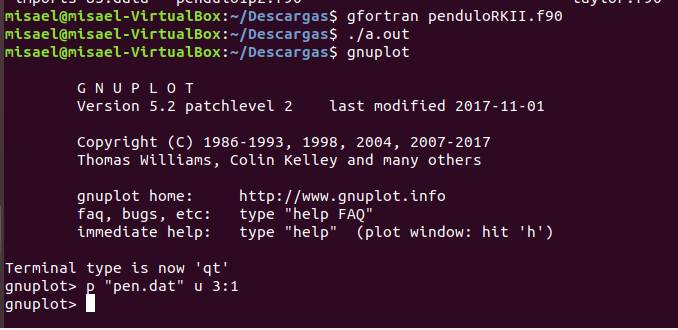
\includegraphics[scale=0.8]{1.PNG}
\end{figure}

\begin{figure}[h!]
    \centering
    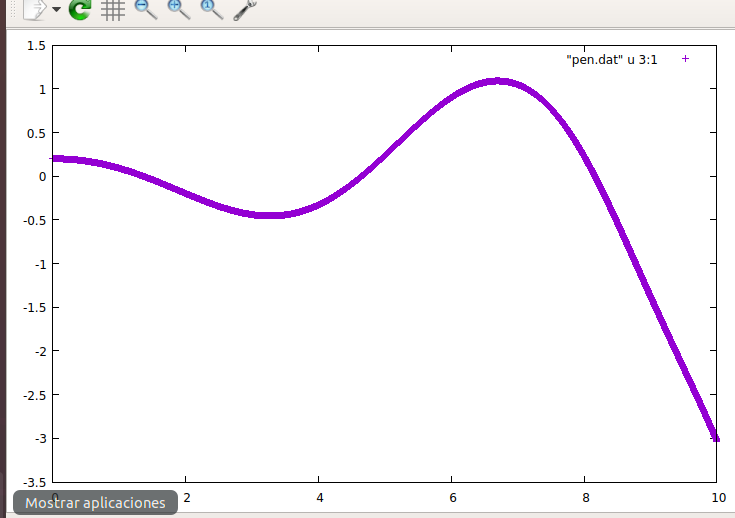
\includegraphics[scale=0.8]{RKII.PNG}
\end{figure}

\newpage

\vspace{5cm}

\begin{verbatim}
PROGRAM Euler_Cromer (código reciclado xd)
!*********************************************************************
! Se resuelve el pendulo no-lineal, amortiguado y con forzamiento
!
!
!**********************************************************************

 REAL*8, DIMENSION(:), ALLOCATABLE :: theta,omega,t
 REAL*8 :: length,dt
!

 !print*,"numero de pasos"
 !read*, n   
 n = 10000
 ALLOCATE (theta(0:n),omega(0:n),t(0:n))
!
!
 call inicializa(theta, omega, t, n, length, dt)
 call calcula (theta, omega, t, n, length, dt)
 call despliega (theta, omega, t, n, length, dt)
!
END PROGRAM Euler_Cromer
!
!
SUBROUTINE inicializa(theta, omega, t, n ,length, dt)
 INTEGER, INTENT (IN) :: n
 REAL*8, DIMENSION(0:n) :: theta,omega,t
 REAL*8 :: length,dt
 !print*,'Angulo inicial del pendulo (en radianes)'
 !read*, theta(0)
 theta(0) = 0.2d0
 !print*,'Velocidad angular inicial del pendulo (en radianes/s)'
 !read*, omega(0)
 omega(0) = 0.d0
 t(0)=0.d0
 !print*,'Longitud del pendulo (in m)'
 !read*, length
 length = 9.80d0
 !print*, 'Tamaño de paso (en segundos)'
 !read*, dt
 dt=0.001
END SUBROUTINE inicializa
!
!
SUBROUTINE calcula(theta, omega, t, n, length, dt)
 INTEGER, INTENT (IN) :: n
 REAL*8, DIMENSION(0:n) :: theta,omega,t
 REAL*8 :: length,dt,g,periodo,k1,k2,k3,k4,l1,l2,l3,l4
 INTEGER :: i
 PI= 4.*ATAN(1.)
 i= 0
 g= 9.80d0
 q=1/2.0d0
 !print*," Amplitud de la fuerza"
 !read*, df
 df = 0.d0
 !df=0.0d0, 0.5d0, 1.20d0
 dfr=2/3.d0
 DO
 t(i+1) = t(i) + dt
 k1 = (-1)*(g/length) *sin(theta(i)) * dt  + q * omega(i)*dt+df*sin(dfr*t(i))*dt
 l1 = omega(i) * dt
 k2 = (-1)*(g/length) *sin(theta(i)+(l1*(0.5d0))) * dt  + q * (omega(i)+(k1*(0.5d0)))*dt+df*sin(dfr*(t(i)+dt*(0.5d0)))*dt
 l2 = (omega(i)+(k1*(0.5d0))) * dt
 k3 = (-1)*(g/length) *sin(theta(i)+(l2*(0.5d0))) * dt  + q * (omega(i)+(k2*(0.5d0)))*dt+df*sin(dfr*(t(i)+dt*(0.5d0)))*dt
 l3 = (omega(i)+(k2*(0.5d0))) * dt
 k4 = (-1)*(g/length) *sin(theta(i)+(l3*(0.5d0))) * dt  + q * (omega(i)+(k3*(0.5d0)))*dt+df*sin(dfr*t(i+1))*dt
 l4 = (omega(i)+(k3*(0.5d0))) * dt
 omega(i+1) = omega(i) + (1/6d0)*(k1+2*k2+2*k3+k4)
 theta(i+1) = theta(i) + (1/6d0)*(l1+2*l2+2*l3+l4)
 !omega(i+1) = omega(i) - (g/length) *sin(theta(i)) * dt  + q * omega(i)*dt+df*sin(dfr*t(i))*dt
 !theta(i+1) = theta(i) + omega(i+1) * dt ! Metodo de Cromer
 if (theta(i+1) > PI ) theta(i+1)=theta(i+1)-2.*PI
 if (theta(i+1) < -PI) theta(i+1)=theta(i+1)+2.*PI
 IF (i >= n-1) EXIT
 i=i+1
 ENDDO
END SUBROUTINE calcula
SUBROUTINE despliega(theta, omega, t, n, length, dt)
 INTEGER, INTENT (IN) :: n
 REAL*8, DIMENSION(0:n) :: theta,omega,t
 REAL*8 :: length,dt
 INTEGER :: i
 CHARACTER(LEN=10), PARAMETER :: f1 = '(3ES16.6)'
 CHARACTER(10) :: archivo
 !print*," archivo de datos"
 !read*, archivo
 archivo = "pen.dat"
 OPEN (UNIT=1,FILE=archivo,STATUS='UNKNOWN')
 !
 WRITE(1,f1)(theta(i),omega(i),t(i), i=0,n)
 !
 CLOSE(1)
END SUBROUTINE despliega
\end{verbatim}

\begin{figure}
    \centering
    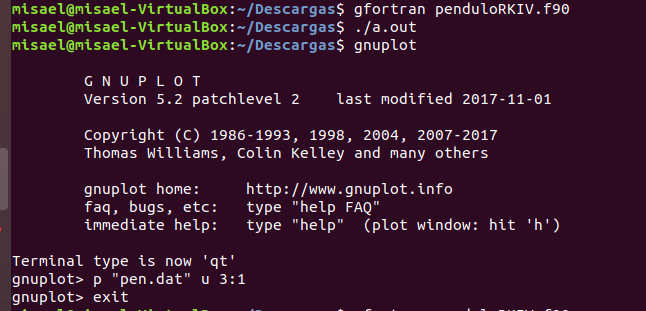
\includegraphics[scale=0.8]{2.PNG}
\end{figure}

\begin{figure}[h]
    \centering
    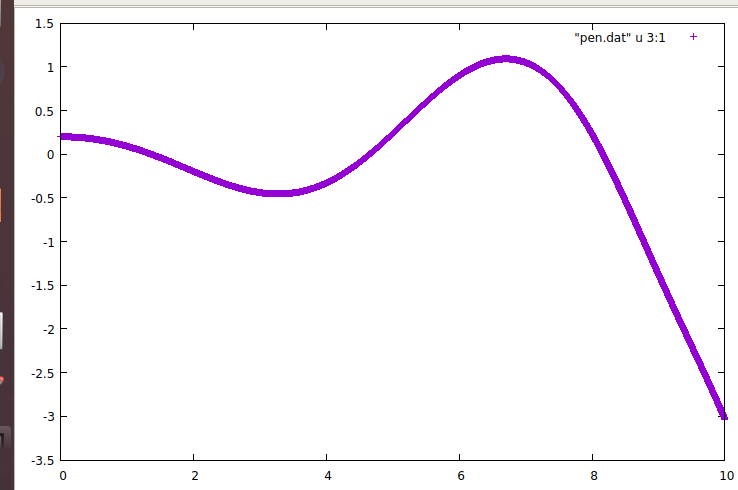
\includegraphics[scale=0.8]{RKIV.PNG}
\end{figure}

\end{document}